% Generated by ic_study.analysis.v4_report_export from the v4 report with
% manifest SHA-256 6608b3960eb73011caca97870a4ffd3dbfbcd4c2df09bbbcb576c1c9452cf981.
% Edited during the journal revision (agent S, 2026-10-13): captions, headers and
% categorical cells in plain English; every number keeps its \resultnum binding.
\begin{figure*}[tp]
\centering
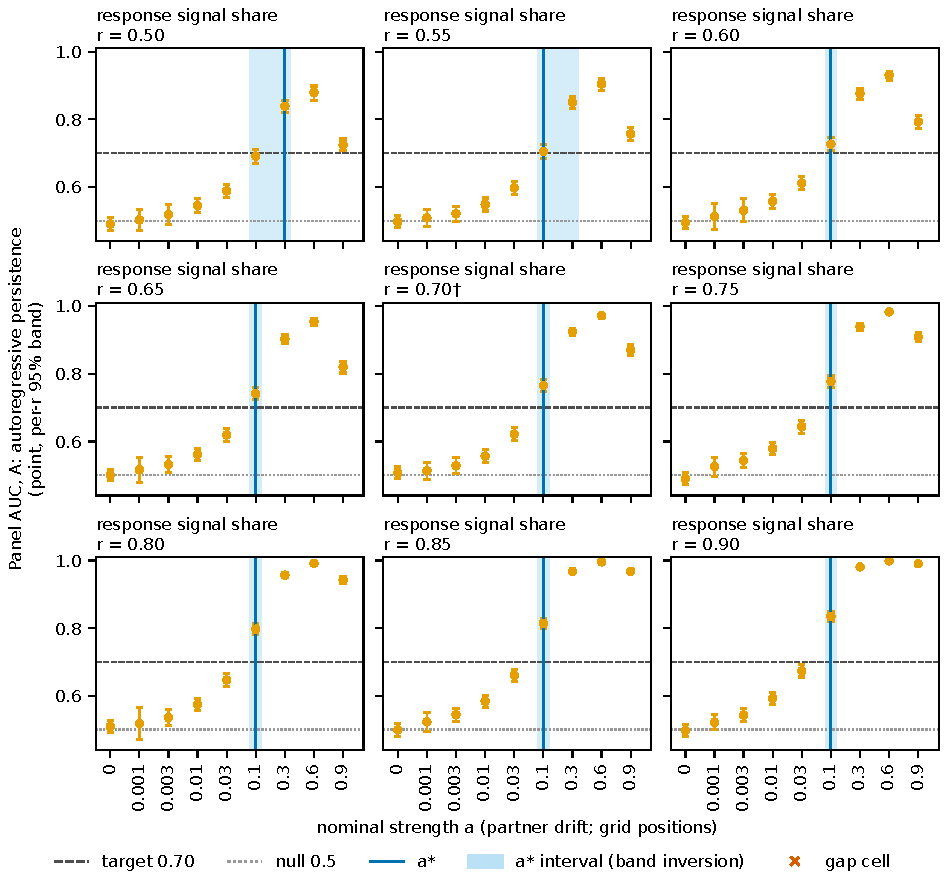
\includegraphics[width=\textwidth,height=175mm,keepaspectratio]{generated/F2_auc_profiles_A.pdf}
\caption{AUC profiles against A (autoregressive persistence), one panel per signal share $r$: point AUC and per-$r$ simultaneous 95\% band at each grid strength of the influence strength $a$ (ordinal positions), the target 0.70 (dashed), 0.5 (dotted), the first boundary $a^*$ (vertical line) and its interval (shaded). Crosses mark fit gaps. The band gives no joint coverage across $r$, models or channels.}\label{fig:v4-F2A}
\end{figure*}
\begin{figure*}[tp]
\centering
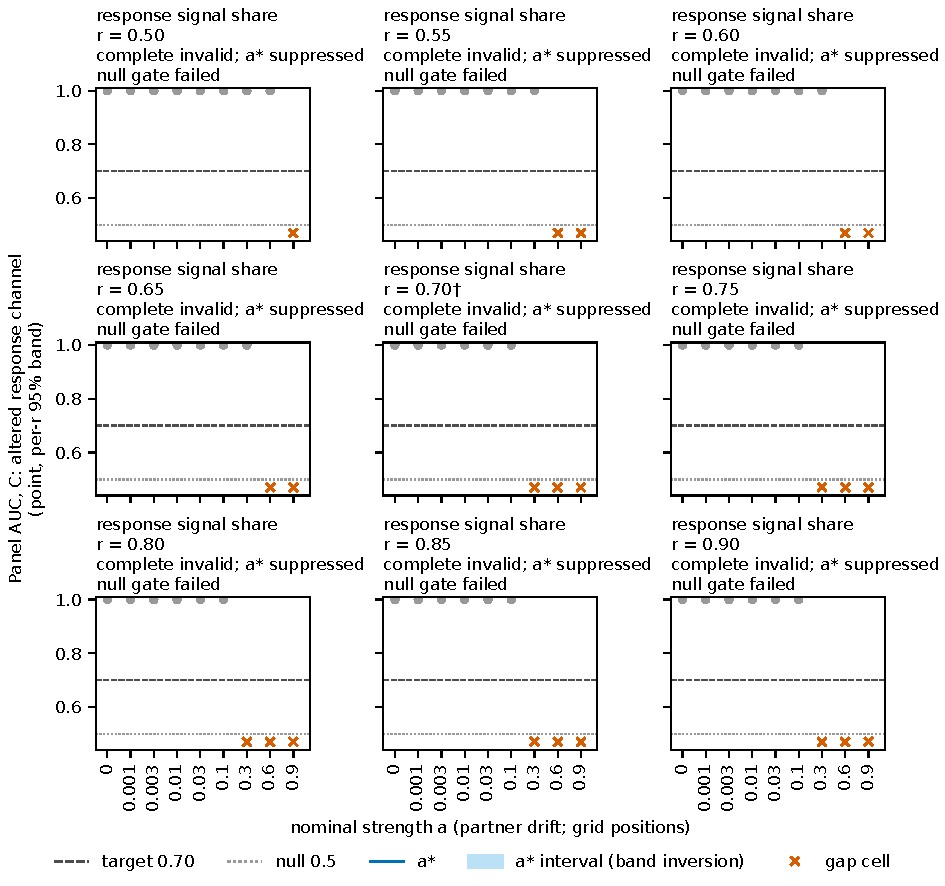
\includegraphics[width=\textwidth,height=175mm,keepaspectratio]{generated/F2_auc_profiles_C.pdf}
\caption{AUC profiles against C (autoregressive persistence with an altered response channel), one panel per signal share $r$: point AUC and per-$r$ simultaneous 95\% band at each grid strength of the influence strength $a$ (ordinal positions), the target 0.70 (dashed), 0.5 (dotted), the first boundary $a^*$ (vertical line) and its interval (shaded). Crosses mark fit gaps. The band gives no joint coverage across $r$, models or channels. In every C unit the point AUC is close to 1 at every strength, $a=0$ included, so the zero-strength check failed at every $r$; points of these invalid units are drawn in gray and no boundary is computed.}\label{fig:v4-F2C}
\end{figure*}
\begin{figure*}[tp]
\centering
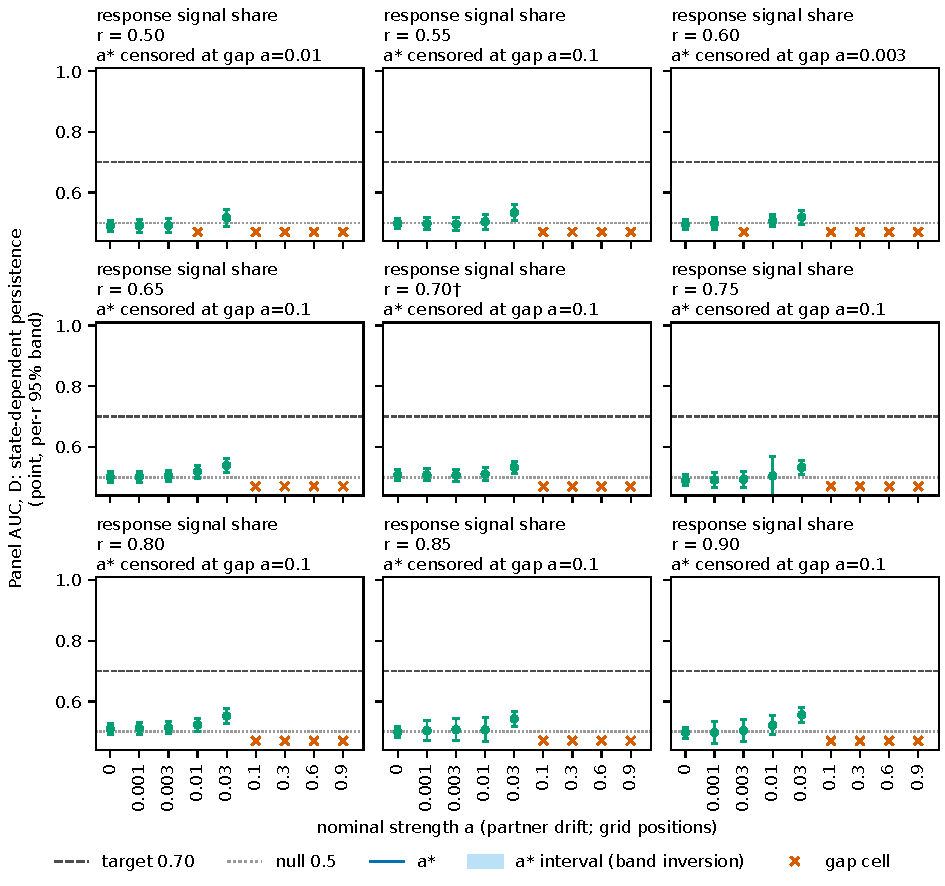
\includegraphics[width=\textwidth,height=175mm,keepaspectratio]{generated/F2_auc_profiles_D.pdf}
\caption{AUC profiles against D (state-dependent persistence), one panel per signal share $r$: point AUC and per-$r$ simultaneous 95\% band at each grid strength of the influence strength $a$ (ordinal positions), the target 0.70 (dashed), 0.5 (dotted), the first boundary $a^*$ (vertical line) and its interval (shaded). Crosses mark fit gaps. The band gives no joint coverage across $r$, models or channels. Crosses mark the fit gaps that censor every D boundary: family limits on the profile at $a=0.10$ and 0.30 at every $r$ and at most higher strengths, a solver gap at $a=0.01$ for $r=0.50$, and the propagation gap at $a=0.003$ for $r=0.60$.}\label{fig:v4-F2D}
\end{figure*}
\begin{figure*}[tp]
\centering
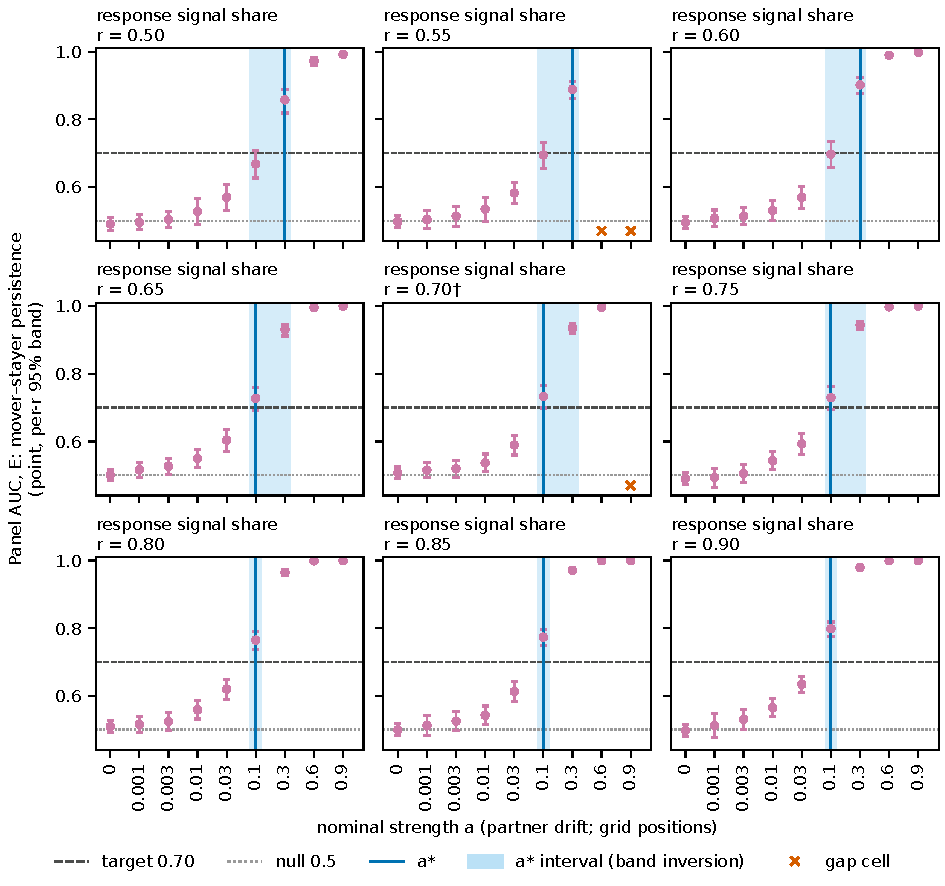
\includegraphics[width=\textwidth,height=175mm,keepaspectratio]{generated/F2_auc_profiles_E.pdf}
\caption{AUC profiles against E (mover--stayer persistence), one panel per signal share $r$: point AUC and per-$r$ simultaneous 95\% band at each grid strength of the influence strength $a$ (ordinal positions), the target 0.70 (dashed), 0.5 (dotted), the first boundary $a^*$ (vertical line) and its interval (shaded). Crosses mark fit gaps. The band gives no joint coverage across $r$, models or channels.}\label{fig:v4-F2E}
\end{figure*}
